Consider a robot capable of motion, equipped with a Light Detection and Ranging
sensor (LIDAR), capturing a measurement $\mathcal{S}_0$ at time $t_0$ from pose
$\bm{p}_0$ in some reference frame. The robot then moves to pose $\bm{p}_1$ at
time $t_1$ at which time it captures measurement $\mathcal{S}_1$. Provided
overlap between the two scans, estimating the rigid-body transformation
$\bm{T}$ that projects the endpoints of $\mathcal{S}_1$ to those of
$\mathcal{S}_0$ with the least error is known as scan-matching. The solution to
the scan-matching problem is central to methods of Localisation, Navigation
\cite{am_odom_4}-\cite{am_odom_6}, and Simultaneous Localisation and Mapping
(SLAM) \cite{am_odom_1}-\cite{am_odom_3}, as $\bm{T}$ is the rigid-body
transformation $\bm{p}_1 - \bm{p}_0$: i.e. the solution to scan-matching
provides localisation information at time $t_1$, relative to $\bm{p}_0$. For
this reason, along with the high measurement accuracy of LIDAR measurements,
scan-matching is also used as a means to improving, providing, or substituting
odometric measurements (where available), as the latter are prone to unbounded
and unpredictable tire and wheel slippage.

LIDAR sensors with a field of view of $360^\circ$, i.e. panoramic sensors, were
for years constrained to high price ranges, and most provided 3D measurements.
Therefore research on scan-matching with 2D LIDAR sensors mostly focused on
non-panoramic sensors, with scan matching methods being used without distinction
with regard to field of view. In recent years, however, price-appealing
2D LIDAR sensors have emerged, but at the cost of increased measurement
uncertainty. The introduction of these sensors warrants targetted research
into scan-matching with the use of panoramic LIDAR sensors, due to (a) the
afforded periodicity of the range signal, and (b) the need of
addressing the high levels of measurement noise with regard to the
transformation errors of current scan-matching algorithms.

This paper introduces a method specifically targeting the matching of 2D
panoramic range scans, whose error is invariant to angular and
locational displacement for a given level of measurement noise.
The central contributions of the paper are:

\begin{itemize}
  \item The use of the Discrete Fourier transform, its properties, and its
        afforded robustness in both orientation and location estimation
        components of the proposed method
  \item The extrication from the need of a prior
  \item The implementation of a method for reducing the orientation error to
        lower than the sensor's angle increment
  \item The parameter set needed by the proposed method is intuitive and smaller
        than those of established methods
  \item The thorough evaluation of the proposed method against two established
        scan-matching algorithms in common use
\end{itemize}

\begin{figure}[]\centering
  \vspace{-1.7cm}
  % GNUPLOT: LaTeX picture with Postscript
\begingroup
  \makeatletter
  \providecommand\color[2][]{%
    \GenericError{(gnuplot) \space\space\space\@spaces}{%
      Package color not loaded in conjunction with
      terminal option `colourtext'%
    }{See the gnuplot documentation for explanation.%
    }{Either use 'blacktext' in gnuplot or load the package
      color.sty in LaTeX.}%
    \renewcommand\color[2][]{}%
  }%
  \providecommand\includegraphics[2][]{%
    \GenericError{(gnuplot) \space\space\space\@spaces}{%
      Package graphicx or graphics not loaded%
    }{See the gnuplot documentation for explanation.%
    }{The gnuplot epslatex terminal needs graphicx.sty or graphics.sty.}%
    \renewcommand\includegraphics[2][]{}%
  }%
  \providecommand\rotatebox[2]{#2}%
  \@ifundefined{ifGPcolor}{%
    \newif\ifGPcolor
    \GPcolorfalse
  }{}%
  \@ifundefined{ifGPblacktext}{%
    \newif\ifGPblacktext
    \GPblacktexttrue
  }{}%
  % define a \g@addto@macro without @ in the name:
  \let\gplgaddtomacro\g@addto@macro
  % define empty templates for all commands taking text:
  \gdef\gplbacktext{}%
  \gdef\gplfronttext{}%
  \makeatother
  \ifGPblacktext
    % no textcolor at all
    \def\colorrgb#1{}%
    \def\colorgray#1{}%
  \else
    % gray or color?
    \ifGPcolor
      \def\colorrgb#1{\color[rgb]{#1}}%
      \def\colorgray#1{\color[gray]{#1}}%
      \expandafter\def\csname LTw\endcsname{\color{white}}%
      \expandafter\def\csname LTb\endcsname{\color{black}}%
      \expandafter\def\csname LTa\endcsname{\color{black}}%
      \expandafter\def\csname LT0\endcsname{\color[rgb]{1,0,0}}%
      \expandafter\def\csname LT1\endcsname{\color[rgb]{0,1,0}}%
      \expandafter\def\csname LT2\endcsname{\color[rgb]{0,0,1}}%
      \expandafter\def\csname LT3\endcsname{\color[rgb]{1,0,1}}%
      \expandafter\def\csname LT4\endcsname{\color[rgb]{0,1,1}}%
      \expandafter\def\csname LT5\endcsname{\color[rgb]{1,1,0}}%
      \expandafter\def\csname LT6\endcsname{\color[rgb]{0,0,0}}%
      \expandafter\def\csname LT7\endcsname{\color[rgb]{1,0.3,0}}%
      \expandafter\def\csname LT8\endcsname{\color[rgb]{0.5,0.5,0.5}}%
    \else
      % gray
      \def\colorrgb#1{\color{black}}%
      \def\colorgray#1{\color[gray]{#1}}%
      \expandafter\def\csname LTw\endcsname{\color{white}}%
      \expandafter\def\csname LTb\endcsname{\color{black}}%
      \expandafter\def\csname LTa\endcsname{\color{black}}%
      \expandafter\def\csname LT0\endcsname{\color{black}}%
      \expandafter\def\csname LT1\endcsname{\color{black}}%
      \expandafter\def\csname LT2\endcsname{\color{black}}%
      \expandafter\def\csname LT3\endcsname{\color{black}}%
      \expandafter\def\csname LT4\endcsname{\color{black}}%
      \expandafter\def\csname LT5\endcsname{\color{black}}%
      \expandafter\def\csname LT6\endcsname{\color{black}}%
      \expandafter\def\csname LT7\endcsname{\color{black}}%
      \expandafter\def\csname LT8\endcsname{\color{black}}%
    \fi
  \fi
    \setlength{\unitlength}{0.0500bp}%
    \ifx\gptboxheight\undefined%
      \newlength{\gptboxheight}%
      \newlength{\gptboxwidth}%
      \newsavebox{\gptboxtext}%
    \fi%
    \setlength{\fboxrule}{0.5pt}%
    \setlength{\fboxsep}{1pt}%
\begin{picture}(5000.00,5000.00)%
    \gplgaddtomacro\gplbacktext{%
      \colorrgb{0.15,0.15,0.15}%
      \put(391,1564){\makebox(0,0)[r]{\strut{}$6.0$}}%
      \colorrgb{0.15,0.15,0.15}%
      \put(391,1988){\makebox(0,0)[r]{\strut{}$8.0$}}%
      \colorrgb{0.15,0.15,0.15}%
      \put(391,2413){\makebox(0,0)[r]{\strut{}$10.0$}}%
      \colorrgb{0.15,0.15,0.15}%
      \put(391,2837){\makebox(0,0)[r]{\strut{}$12.0$}}%
      \colorrgb{0.15,0.15,0.15}%
      \put(391,3262){\makebox(0,0)[r]{\strut{}$14.0$}}%
      \colorrgb{0.15,0.15,0.15}%
      \put(391,3687){\makebox(0,0)[r]{\strut{}$16.0$}}%
      \colorrgb{0.00,0.00,0.00}%
      \put(672,1280){\makebox(0,0){\strut{}$-2.0$}}%
      \colorrgb{0.00,0.00,0.00}%
      \put(1096,1280){\makebox(0,0){\strut{}$0.0$}}%
      \colorrgb{0.00,0.00,0.00}%
      \put(1521,1280){\makebox(0,0){\strut{}$2.0$}}%
      \colorrgb{0.00,0.00,0.00}%
      \put(1945,1280){\makebox(0,0){\strut{}$4.0$}}%
      \colorrgb{0.00,0.00,0.00}%
      \put(2370,1280){\makebox(0,0){\strut{}$6.0$}}%
    }%
    \gplgaddtomacro\gplfronttext{%
    }%
    \gplgaddtomacro\gplbacktext{%
      \colorrgb{0.00,0.00,0.00}%
      \put(2822,1280){\makebox(0,0){\strut{}$-2.0$}}%
      \colorrgb{0.00,0.00,0.00}%
      \put(3246,1280){\makebox(0,0){\strut{}$0.0$}}%
      \colorrgb{0.00,0.00,0.00}%
      \put(3671,1280){\makebox(0,0){\strut{}$2.0$}}%
      \colorrgb{0.00,0.00,0.00}%
      \put(4095,1280){\makebox(0,0){\strut{}$4.0$}}%
      \colorrgb{0.00,0.00,0.00}%
      \put(4520,1280){\makebox(0,0){\strut{}$6.0$}}%
    }%
    \gplgaddtomacro\gplfronttext{%
    }%
    \gplbacktext
    \put(0,0){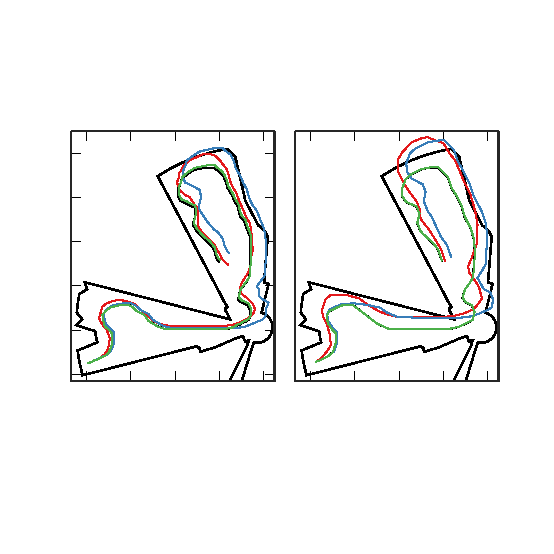
\includegraphics{./figures/odom_test_5_vs_6}}%
    \gplfronttext
  \end{picture}%
\endgroup

  \vspace{-2.3cm}
  \caption{\small Scan-matching as ``laser odometry": the robot moves from the
           lower left portion of the environment to the upper right, capturing
           2D range scans along its trajectory (black). The red (CSM), blue
           (NDT), and green (our method) routes show the estimated path of the
           robot derived from each method. Left figure: frequent LIDAR
           measurements.  Right figure: a downsampled version of the original
           trajectory. The proposed method's error is invariant to angular and
           locational displacement}
  \label{fig:laser_odometry}
\end{figure}

The rest of the paper is structured as follows. Section
\ref{section:definitions} defines necessary notions.  The problem of matching
panoramic 2D range scans is formulated in section \ref{section:the_problem},
and a brief review of methods matching 2D range scans is given in section
\ref{section:sota}. Section \ref{section:the_proposed_method} provides an
analysis of the proposed method. The experimental setup and results of the
proposed method against two methods in common use are illustrated in section
\ref{section:results}. Section \ref{section:finale} offers a recapitulation.
